% homework/hw02/hw02.tex
% Year 7 - Homework Packet 2
% Covers Maths 1.2 (multiplying and dividing integers), Maths 1.3 (multiples
% and the LCM), Science 1.2 (comparing plant and animal cells) and Science 1.3
% (specialised cells).
%
% House style is shared: see homework/hw-style.tex. Method: the new-homework
% skill. Source is pure ASCII on purpose.
%
% Build:  pwsh .claude/skills/new-homework/scripts/build-hw.ps1 hw02

\documentclass[12pt,a4paper]{article}

% -- Answer key switch -------------------------------------------------------
\newif\ifkey
\ifdefined\TEACHER\keytrue\else
  \keyfalse        % \keyfalse = student copy   |   \keytrue = teacher copy
\fi

% -- House style -------------------------------------------------------------
% homework/hw-style.tex
% Shared house style for every Year 7 homework packet. \input this from the
% packet file, right after \documentclass and the answer-key switch.
%
% Do not fork this file per packet. If a packet needs a different look, the
% question is whether every packet should have it.
%
% The choices here are deliberate and were arrived at by printing and looking:
%   * No solid dark banners. Every header is a light tint with a coloured spine
%     on the left, so colour reads clearly without flooding a school printer.
%   * No marks and no mark totals. These are practice, not exam papers.
%   * Lato at 12pt with open leading, plus mathastext so inline maths is Lato
%     too. Without mathastext every "-6 + 4" is Computer Modern serif and the
%     sheet looks half-typeset.
%   * Writing lines are spaced for Year 7 handwriting, not adult margin notes.
%
% Provides: \wlines \blank \tickbox \sep \qmk-free marks (none) \hwsection
% \qhead \expr, the workspace box, and the remember / wordhelp / activity /
% yourturn coloured boxes. Palette matches the lesson decks exactly.

% -- Packages ----------------------------------------------------------------
\usepackage[T1]{fontenc}
\usepackage[utf8]{inputenc}
\usepackage[default]{lato}
\usepackage[a4paper,top=1.7cm,bottom=1.7cm,left=2.0cm,right=2.0cm,headheight=15pt]{geometry}
\usepackage{amsmath,amssymb}
\usepackage{xcolor}
\usepackage[most]{tcolorbox}
\usepackage{enumitem}
\usepackage{tikz}
\usetikzlibrary{arrows.meta}
\usepackage{array}
\usepackage{tabularx}
\usepackage{fancyhdr}
\usepackage{multicol}
\usepackage{needspace}
\usepackage{graphicx}

% Make maths use Lato too. Without this, every "-6 + 4" on the page is set in
% Computer Modern serif and the sheet looks half-typeset. Must come last.
\usepackage[italic]{mathastext}

\linespread{1.06}\selectfont

% -- The Learner's Book palette (same hex values as the lesson decks) ---------
\definecolor{cbteal}{HTML}{0087A8}
\definecolor{cbpurple}{HTML}{5C2483}
\definecolor{cborange}{HTML}{C25E12}
\definecolor{cbgreen}{HTML}{4A8B23}
\definecolor{cbred}{HTML}{C8102E}
\definecolor{cbblue}{HTML}{1A5FA8}
\definecolor{rulegray}{HTML}{9AA5AD}

% -- Answer lines and blanks -------------------------------------------------
% \wlines{n} draws n ruled writing lines, spaced wide enough for Year 7
% handwriting rather than for an adult with a fine pen.
\makeatletter
\newcommand{\wlines}[1]{%
  \par\vspace{0.75em}%
  \@tempcnta=0\relax
  \@whilenum\@tempcnta<#1\do{%
    \hbox to \linewidth{\color{rulegray}\leaders\hrule height 0.5pt\hfill}%
    \vspace{1.5em}%
    \advance\@tempcnta by 1\relax}%
  \par\vspace{-0.8em}%
}
\makeatother

% \blank[width] is an inline gap to write a short answer in.
\newcommand{\blank}[1][2.6cm]{\underline{\hspace{#1}}}

% A boxed space for showing working.
\newtcolorbox{workspace}[1][3.4cm]{%
  colback=white, colframe=rulegray, boxrule=0.5pt, arc=5pt,
  height=#1, left=6pt, right=6pt, top=4pt, bottom=4pt,
  before skip=9pt, after skip=11pt}

% An empty tick box.
\newcommand{\tickbox}{\fbox{\rule{0pt}{1.15em}\rule{1.15em}{0pt}}}

% A middot separator.
\newcommand{\sep}{\,\textperiodcentered\,}

% -- Section and question headings -------------------------------------------
% Light tint plus a fat coloured spine on the left. No solid dark banner: the
% colour reads clearly but barely costs the printer anything.
% needspace stops a heading stranding alone at the foot of a page. Kept modest:
% too large and it pushes headings over, leaving a worse hole than it prevents.
\newcommand{\hwsection}[2][cbteal]{%
  \needspace{8\baselineskip}%
  \par\vspace{13pt}%
  \noindent
  \begin{tcolorbox}[enhanced, nobeforeafter, width=\textwidth,
      colback=#1!7, colframe=#1!7, arc=5pt,
      borderline west={5pt}{0pt}{#1},
      left=14pt, right=10pt, top=7pt, bottom=7pt]
    {\large\bfseries\color{#1}#2}
  \end{tcolorbox}%
  \par\vspace{9pt}}

% \qhead[colour]{A2}{Moving along the line} -- a question heading.
\newcommand{\qhead}[3][cbteal]{%
  \needspace{6\baselineskip}%
  \par\vspace{11pt}%
  \noindent{\large\bfseries\color{#1}#2}\quad{\large\bfseries #3}\par\vspace{4pt}}

% -- Coloured boxes ----------------------------------------------------------
% Shared look: rounded, light fill, coloured rule, coloured title text on a
% pale title strip rather than a dark one.
\tcbset{hwbox/.style={
  enhanced, breakable, arc=6pt, boxrule=1pt,
  left=11pt, right=11pt, top=8pt, bottom=8pt,
  fonttitle=\bfseries, attach boxed title to top left={xshift=12pt, yshift=-8pt},
  boxed title style={arc=4pt, boxrule=1pt, left=7pt, right=7pt, top=2pt, bottom=2pt},
  top=13pt}}

% Orange: things to remember. Matches the deck's "Write This Down".
\newtcolorbox{remember}[1][Remember from the lesson]{hwbox,
  colback=cborange!6, colframe=cborange, coltitle=cborange,
  colbacktitle=white, title={#1}}

% Blue: English help. The barrier in this class is the wording, not the maths.
\newtcolorbox{wordhelp}[1][Word help]{hwbox,
  colback=cbblue!6, colframe=cbblue, coltitle=cbblue,
  colbacktitle=white, title={#1}}

% Purple: an activity or instruction.
\newtcolorbox{activity}[1][How to do this homework]{hwbox,
  colback=cbpurple!6, colframe=cbpurple, coltitle=cbpurple,
  colbacktitle=white, title={#1}}

% Green: your turn / a friendly nudge.
\newtcolorbox{yourturn}[1][Your turn]{hwbox,
  colback=cbgreen!7, colframe=cbgreen, coltitle=cbgreen!75!black,
  colbacktitle=white, title={#1}}

% -- Shorthands --------------------------------------------------------------
\newcommand{\dC}{\,^{\circ}\mathrm{C}}          % use inside maths: $-8\dC$
\newcommand{\key}[1]{{\color{cborange}\textbf{#1}}}
\newcommand{\eng}[1]{{\color{cbblue}\textbf{#1}}}

\setlist[enumerate]{itemsep=8pt, topsep=5pt, leftmargin=*}
\setlist[itemize]{itemsep=4pt, topsep=4pt, leftmargin=*}
\renewcommand{\arraystretch}{1.45}

% -- An expression the student is asked to work from -------------------------
\newcommand{\expr}[1]{%
  \tcbox[on line, colback=cbgreen!10, colframe=cbgreen!55, boxrule=1pt, arc=4pt,
         left=9pt, right=9pt, top=4pt, bottom=4pt]{\large\bfseries $#1$}}

% -- Running head and foot ---------------------------------------------------
% The packet overrides \fancyhead[L] with its own title.
\pagestyle{fancy}
\fancyhf{}
\fancyhead[L]{\small\color{black!55}Year 7\sep Homework}
\fancyhead[R]{\small\color{black!55}Name: \blank[3.4cm]}
\fancyfoot[C]{\small\color{black!55}Page \thepage}
\renewcommand{\headrulewidth}{0pt}
\renewcommand{\headrule}{\vspace{2pt}\hbox to\headwidth{\color{cbteal!45}\leaders\hrule height 1.2pt\hfill}}



% -- Per-packet running head -------------------------------------------------
\fancyhead[L]{\small\color{black!55}Year 7\sep Homework 2}

\begin{document}

% ===========================================================================
% COVER BLOCK
% ===========================================================================
\thispagestyle{fancy}

\begin{tcolorbox}[enhanced, colback=cbpurple!7, colframe=cbpurple!7, arc=7pt,
                  borderline west={6pt}{0pt}{cbpurple},
                  left=18pt, right=14pt, top=14pt, bottom=14pt]
  {\color{cbpurple}\bfseries YEAR 7\sep UNIT 1\sep HOMEWORK 2}\\[6pt]
  {\color{cbpurple}\Huge\bfseries Signs, Multiples and Cells}\\[10pt]
  {\color{black!70}Mathematics 1.2 --- Multiplying \& Dividing Integers\sep
   1.3 --- Multiples and the LCM}\\
  {\color{black!70}Science 1.2 --- Plant \& Animal Cells\sep
   1.3 --- Specialised Cells}
\end{tcolorbox}

\vspace{10pt}
\noindent
\begin{tabularx}{\textwidth}{@{}X X@{}}
  \textbf{Name:} \blank[5.6cm] & \textbf{Class:} \blank[5.6cm] \\
  \textbf{Date given:} \blank[4.6cm] & \textbf{Date due:} \blank[5.0cm] \\
\end{tabularx}

\vspace{8pt}
\begin{activity}
  \begin{itemize}
    \item Write your answers \textbf{on this sheet}, in the spaces given. If you need
          more room, use the back of the page.
    \item In maths, \key{write the calculation before the answer}.
    \item In science, answer in \key{full English sentences}. ``Haemoglobin'' is not a
          sentence; ``A red blood cell is full of haemoglobin'' is.
    \item If a word is new to you, look for the blue \eng{Word help} box on that page
          before you give up.
  \end{itemize}
\end{activity}

% ===========================================================================
% SECTION A -- MATHS 1.2
% ===========================================================================
\hwsection{Section A \textperiodcentered\ Mathematics 1.2 --- Multiplying and Dividing Integers}

\begin{remember}
  \key{Same signs give a positive. Different signs give a negative.} The same four
  rules work for \key{$\times$} and for \key{$\div$}, because dividing undoes
  multiplying.

  \medskip
  A \key{product} is the answer when you multiply. The product of 2 and $-9$ is $-18$.
\end{remember}

% -- A1 ---------------------------------------------------------------------
\qhead{A1}{The four rules}

\noindent\textbf{(a)} Fill in the sign that each rule gives you.

\vspace{10pt}
\noindent\hspace*{1em}
\begin{tabular}{@{}l@{\hspace{1.4cm}}l@{\hspace{1.4cm}}l@{\hspace{1.4cm}}l@{}}
  $+ \times + = \blank[1.1cm]$ &
  $+ \times - = \blank[1.1cm]$ &
  $- \times + = \blank[1.1cm]$ &
  $- \times - = \blank[1.1cm]$ \\
\end{tabular}

\vspace{12pt}
\noindent\textbf{(b)} Now work these out.

\vspace{8pt}
\begin{multicols}{3}
\begin{enumerate}[label=(\alph*), itemsep=13pt]
  \item $-6 \times 4 = \blank[1.5cm]$
  \item $7 \times -3 = \blank[1.5cm]$
  \item $-5 \times -8 = \blank[1.5cm]$
  \item $-36 \div 6 = \blank[1.5cm]$
  \item $45 \div -9 = \blank[1.5cm]$
  \item $-56 \div -7 = \blank[1.5cm]$
  \item $-9 \times 0 = \blank[1.5cm]$
  \item $-12 \div -12 = \blank[1.5cm]$
  \item $8 \times -7 = \blank[1.5cm]$
  \item $-3 \times -3 = \blank[1.5cm]$
  \item $-100 \div 4 = \blank[1.5cm]$
  \item $-60 \div -5 = \blank[1.5cm]$
\end{enumerate}
\end{multicols}

% -- A2 ---------------------------------------------------------------------
\qhead{A2}{Say it, then write it}

\begin{wordhelp}[Word help --- the English decides which number comes first]
  \begin{tabularx}{\linewidth}{@{}lX@{}}
    \eng{multiply $-7$ by 6}   & you \textbf{start} at $-7$: $-7 \times 6$. \\
    \eng{divide $-40$ by 8}    & you start at $-40$: $-40 \div 8$. \\
    \eng{5 divided into $-35$} & the same trap as last week --- it is $-35 \div 5$, not $5 \div -35$. \\
    \eng{the product of}       & the answer when you \textbf{multiply}. \\
    \eng{times}                & the everyday English word for multiply. \\
    \eng{share equally between}& divide. \\
  \end{tabularx}
\end{wordhelp}

\noindent Turn each sentence into a calculation, then work out the answer.
\key{Write the calculation first.}

\vspace{6pt}
\begin{enumerate}[label=\arabic*., itemsep=11pt]
  \item Multiply $-7$ by 6. \\[4pt]
        Calculation: \blank[6.2cm] \quad Answer: \blank[2.4cm]
  \item Divide $-40$ by 8. \\[4pt]
        Calculation: \blank[6.2cm] \quad Answer: \blank[2.4cm]
  \item What is the product of $-9$ and $-4$? \\[4pt]
        Calculation: \blank[6.2cm] \quad Answer: \blank[2.4cm]
  \item 5 divided into $-35$. \\[4pt]
        Calculation: \blank[6.2cm] \quad Answer: \blank[2.4cm]
  \item Mr Bowen shares a debt of 24 dollars equally between 6 people. Write each
        person's share as a negative number. \\[4pt]
        Calculation: \blank[6.2cm] \quad Answer: \blank[2.4cm]
\end{enumerate}

% -- A3 ---------------------------------------------------------------------
\qhead[cbgreen]{A3}{A sentence that is only half true}

\begin{yourturn}[Think carefully about this one]
  People often say: \textbf{``Two negatives make a positive.''}

  \medskip
  It is a useful sentence, but it is only true \emph{sometimes}. Test it yourself
  before you decide.
\end{yourturn}

\noindent\textbf{(a)} Work out \quad \expr{-3 \times -4} \quad Answer: \blank[2.4cm]

\vspace{8pt}
\noindent\textbf{(b)} Work out \quad \expr{-3 + -4} \quad Answer: \blank[2.4cm]

\vspace{10pt}
\noindent\textbf{(c)} Is ``two negatives make a positive'' true for \textbf{both} of
them? Answer in one full sentence.
\wlines{2}

\vspace{6pt}
\noindent\textbf{(d)} Rewrite the sentence so that it is \textbf{always} true. You will
need to say which operations it works for.
\wlines{2}

% -- A4 ---------------------------------------------------------------------
\qhead{A4}{Brackets, and checking yourself}

\begin{remember}[Two rules that save marks]
  \key{Do the brackets first.} Work out what is inside, then multiply or divide.
  Careful: if the bracket holds an \key{addition}, the sign rules above do
  \key{not} apply inside it.

  \medskip
  \key{Estimate:} round each number to something easy, calculate, and check your real
  answer is close to it.
\end{remember}

\noindent\textbf{(a)} Work these out. Show what the bracket comes to first.

\vspace{6pt}
\begin{enumerate}[label=(\roman*), itemsep=11pt]
  \item $20 \div (-3 + -2) = \blank[2.4cm]$
  \item $(-4 + 10) \times -3 = \blank[2.4cm]$
  \item $-6 \times (2 - 9) = \blank[2.4cm]$
\end{enumerate}

\vspace{8pt}
\noindent\textbf{(b)} \textbf{Estimate} each of these by rounding first. Write the
rounded calculation as well as the answer.

\vspace{6pt}
\begin{enumerate}[label=(\roman*), itemsep=6pt, start=4]
  \item $-6.2 \times 3.9$ \quad is about \blank[3.4cm] $= \blank[2.2cm]$
  \item $62 \div -7.8$ \quad is about \blank[3.4cm] $= \blank[2.2cm]$
\end{enumerate}

% -- A5 ---------------------------------------------------------------------
\qhead{A5}{Word problems}

\noindent Read each one \key{all the way to the end} before you start writing.

\begin{enumerate}[label=\textbf{\arabic*.}, itemsep=14pt]

  \item \textbf{The monthly fee.} Mr Bowen's bank takes a 4-dollar fee out of his
        account at the end of every month. He forgets about it for 7 months. What is
        the total change to his balance?
        \begin{workspace}[2.8cm]\end{workspace}

  \item \textbf{The dive.} A submarine starts at the surface and descends steadily.
        After 6 minutes it is at $-54$ m. How far does it travel each minute?
        \begin{workspace}[2.8cm]\end{workspace}

  \item \textbf{The market stall.} Mr Bowen takes 47 identical rubber ducks to the
        market to sell. He plans to sell them for 3 dollars each, and the market
        charges him a 2-dollar fee on every duck he sells, plus 15 dollars for the
        stall. It rains all day and nobody comes, so he sells 0 ducks. How much money
        does he make or lose that day?
        \begin{workspace}[3.1cm]\end{workspace}

\end{enumerate}

% ===========================================================================
% SECTION B -- MATHS 1.3
% ===========================================================================
\hwsection{Section B \textperiodcentered\ Mathematics 1.3 --- Multiples and the LCM}

\begin{remember}
  A \key{multiple} is the answer when you multiply a number by 1, 2, 3, 4, \ldots
  The multiples of 4 are 4, 8, 12, 16, 20, \ldots

  \medskip
  In everyday English, \eng{common} means \emph{ordinary}. In maths it means
  \key{shared}. A \key{common multiple} of two numbers is in \key{both} lists, and the
  \key{lowest common multiple (LCM)} is the smallest of them. You already know this
  idea in Vietnamese as \key{BCNN}.
\end{remember}

% -- B1 ---------------------------------------------------------------------
\qhead{B1}{Build it from the lists}

\noindent\textbf{(a)} Write the first six multiples of \textbf{8}.
\vspace{4pt}

\noindent\hspace*{1em}\blank[13cm]

\vspace{10pt}
\noindent\textbf{(b)} Write the first six multiples of \textbf{12}.
\vspace{4pt}

\noindent\hspace*{1em}\blank[13cm]

\vspace{10pt}
\noindent\textbf{(c)} Which numbers appear in \textbf{both} lists? These are the
common multiples.
\vspace{4pt}

\noindent\hspace*{1em}\blank[13cm]

\vspace{10pt}
\noindent\textbf{(d)} So the \textbf{LCM} of 8 and 12 is \blank[3cm]

% -- B2 ---------------------------------------------------------------------
\qhead{B2}{Do not just multiply them}

\begin{remember}[The trap in this topic]
  The LCM is usually \key{smaller} than the two numbers multiplied together.
  If one number \key{divides into} the other, the LCM is just the \key{bigger} number.
  When you are not sure, \key{list them}.
\end{remember}

\noindent Find the LCM of each pair.

\vspace{8pt}
\begin{multicols}{2}
\begin{enumerate}[label=(\alph*), itemsep=12pt]
  \item 3 and 7 \quad LCM $= \blank[2.2cm]$
  \item 5 and 20 \quad LCM $= \blank[2.2cm]$
  \item 6 and 8 \quad LCM $= \blank[2.2cm]$
  \item 9 and 9 \quad LCM $= \blank[2.2cm]$
\end{enumerate}
\end{multicols}

\vspace{6pt}
\noindent\textbf{(e)} A student says the LCM of 5 and 20 is 100, because
$5 \times 20 = 100$. In one full sentence, explain what they have got wrong.
\wlines{2}

% -- B3 ---------------------------------------------------------------------
\qhead{B3}{Word problems}

\begin{enumerate}[label=\textbf{\arabic*.}, itemsep=14pt]

  \item \textbf{The two lighthouses.} One lighthouse flashes every 6 seconds. The
        other flashes every 10 seconds. They have just flashed at the same moment.
        How many seconds until they next flash together?
        \begin{workspace}[2.9cm]\end{workspace}

  \item \textbf{The bread and the cheese.} Mr Bowen is making sandwiches. Bread rolls
        come in packs of 8. Slices of cheese come in packs of 12. He wants one slice
        of cheese in every roll, with nothing left over. What is the smallest number
        of sandwiches he can make, and how many packs of each must he buy?
        \begin{workspace}[3.3cm]\end{workspace}

\end{enumerate}

% -- B4 ---------------------------------------------------------------------
\qhead[cbgreen]{B4}{Now you write the question}

\begin{yourturn}[Your turn to be the teacher]
  So far the questions have given you the English, and you have written the maths.
  Now do it \textbf{backwards}. You are given the maths --- write the English.

  \medskip
  Your word problem must:
  \begin{itemize}
    \item be about something \textbf{real};
    \item be written in \textbf{full English sentences}, and end with a question;
    \item have the answer that is already given to you.
  \end{itemize}
\end{yourturn}

\noindent\textbf{(a)} Write a word problem for \quad \expr{7 \times -4 = -28}
\wlines{4}

\vspace{12pt}
\noindent\textbf{(b)} Write a word problem for \quad \expr{\text{LCM of 4 and 10} = 20}

\vspace{2pt}
{\small\color{black!60}This one must be about two things that keep repeating, and the
question must ask when they next happen together.}
\wlines{4}

% ===========================================================================
% SECTION C -- SCIENCE 1.2
% ===========================================================================
\hwsection{Section C \textperiodcentered\ Science 1.2 --- Comparing Plant and Animal Cells}

\begin{remember}
  An animal cell has a \key{cell membrane}, \key{cytoplasm}, \key{mitochondria} and a
  \key{nucleus}. A plant cell has all four of those \key{plus} a \key{cell wall},
  \key{chloroplasts} and a \key{sap vacuole}.

  \medskip
  The one clue that always works is the \key{cell wall} --- a straight, stiff edge,
  with the cells packed together like bricks. \key{``Not green'' does not mean
  animal.}
\end{remember}

% -- C1 ---------------------------------------------------------------------
\qhead{C1}{Match the word to its meaning}

\noindent Write the correct letter in the box next to each word.

\vspace{8pt}
\noindent
\begin{tabularx}{\textwidth}{@{}p{3.8cm} @{\hspace{6pt}} c @{\hspace{12pt}} X@{}}
  \textbf{Word} & \textbf{Letter} & \textbf{Meaning} \\[2pt]
  1.\ Stain          & \tickbox & \textbf{A} \; The job that a cell does. \\
  2.\ Similar        & \tickbox & \textbf{B} \; The tough substance a cell wall is made of. \\
  3.\ Function       & \tickbox & \textbf{C} \; A coloured dye added to a specimen to make its parts easier to see. \\
  4.\ Specialised    & \tickbox & \textbf{D} \; The green substance inside a chloroplast. \\
  5.\ Cellulose      & \tickbox & \textbf{E} \; Alike in some ways and different in others --- \textbf{not} the same. \\
  6.\ Chlorophyll    & \tickbox & \textbf{F} \; The cell has a structure that helps it do its job really well. \\
\end{tabularx}

% -- C2 ---------------------------------------------------------------------
\qhead{C2}{Plant or animal? And how do you know?}

\noindent Mr Bowen looks at four slides down the microscope. For each one, write
\textbf{plant} or \textbf{animal}, and then give the \textbf{one feature} that tells
you.

\vspace{8pt}
\noindent
\begin{tabularx}{\textwidth}{|c|>{\raggedright\arraybackslash}X|p{2.7cm}|p{4.3cm}|}
  \hline
  & \textbf{What Mr Bowen sees} & \textbf{Plant or animal?} & \textbf{The feature that tells you} \\
  \hline
  1 & Cells with straight, stiff edges, packed together like bricks, and full of small green discs. \rule[-1.1em]{0pt}{2.4em} & & \\ \hline
  2 & Round, separate cells with no straight edges anywhere. \rule[-1.1em]{0pt}{2.4em} & & \\ \hline
  3 & Purple cells with no green discs at all --- but every cell has straight sides. \rule[-1.1em]{0pt}{2.4em} & & \\ \hline
  4 & Long, soft fibres with many dark nuclei, and no straight edges. \rule[-1.1em]{0pt}{2.4em} & & \\ \hline
\end{tabularx}

\vspace{10pt}
\noindent{\small\color{black!60}One of these four catches almost everybody. Read the
orange box at the top of this section again before you answer.}

% -- C3 ---------------------------------------------------------------------
\qhead{C3}{Similar is not the same}

\begin{wordhelp}[Word help --- three patterns for comparing]
  ``A and B are \eng{similar because} both of them \ldots''\\
  ``They are \eng{different because} A has \ldots, \eng{but} B \ldots''\\
  ``\eng{Unlike} an animal cell, a plant cell \ldots''
\end{wordhelp}

\begin{enumerate}[label=\arabic*., itemsep=12pt]
  \item Finish this sentence: ``A plant cell and an animal cell are
        \textbf{similar because} both of them \ldots''
        \wlines{1}
  \item Finish this one: ``They are \textbf{different because} a plant cell has
        \ldots, \textbf{but} an animal cell \ldots''
        \wlines{1}
  \item An animal cell has no fixed shape. Explain why, in one full sentence.
        \wlines{2}
\end{enumerate}

% -- C4 ---------------------------------------------------------------------
\qhead{C4}{Put the method in order}

\noindent These are the steps for making a stained slide of your own cheek cells, but
they are in the wrong order. Number them \textbf{1} to \textbf{6}.

\vspace{10pt}
\noindent
\begin{tabularx}{\textwidth}{|c|X|}
  \hline
  \tickbox \rule{0pt}{1.6em} & Add one drop of methylene blue stain to the sample. \\ \hline
  \tickbox \rule{0pt}{1.6em} & Looking \textbf{from the side}, move the lens down close to the slide. \\ \hline
  \tickbox \rule{0pt}{1.6em} & Rub the inside of your cheek gently with a clean cotton bud. \\ \hline
  \tickbox \rule{0pt}{1.6em} & Look down the eyepiece and turn the focus so the lens moves \textbf{away}, until the cells are sharp. \\ \hline
  \tickbox \rule{0pt}{1.6em} & Lower a cover slip onto the drop slowly, so that no air bubbles are trapped. \\ \hline
  \tickbox \rule{0pt}{1.6em} & Wipe the cotton bud onto the middle of a clean glass slide. \\ \hline
\end{tabularx}

\vspace{12pt}
\noindent Why must you look \textbf{from the side} in one of those steps? Answer in one
full sentence.
\wlines{2}

% ===========================================================================
% SECTION D -- SCIENCE 1.3
% ===========================================================================
\hwsection{Section D \textperiodcentered\ Science 1.3 --- Specialised Cells}

\begin{remember}
  A cell's \key{function} is the job it does. A \key{specialised} or \key{adapted}
  cell has a structure that helps it do that job really well.

  \medskip
  The sentence to use every time:\quad
  A [cell] is \key{adapted to} [its job] \key{because it has} [its special feature].
\end{remember}

% -- D1 ---------------------------------------------------------------------
\qhead{D1}{Finish the table}

\noindent The first row is done for you. Fill in the other four.

\vspace{8pt}
\noindent\small
\begin{tabularx}{\textwidth}{|p{2.5cm}|>{\raggedright\arraybackslash}p{3.2cm}|>{\raggedright\arraybackslash}p{3.2cm}|>{\raggedright\arraybackslash}X|}
  \hline
  \textbf{Name} & \textbf{Function (its job)} & \textbf{Special structure} &
  \textbf{How this helps} \\
  \hline
  Red blood cell \rule[-0.5em]{0pt}{1.6em} & Carries oxygen around the body. &
  Full of haemoglobin, and no nucleus. &
  Haemoglobin holds the oxygen, and losing the nucleus leaves more room for it. \\
  \hline
  Neurone \rule[-2.6em]{0pt}{3.6em} & & & \\
  \hline
  Ciliated cell \rule[-2.6em]{0pt}{3.6em} & & & \\
  \hline
  Root hair cell \rule[-2.6em]{0pt}{3.6em} & & & \\
  \hline
  Palisade cell \rule[-2.6em]{0pt}{3.6em} & & & \\
  \hline
\end{tabularx}
\normalsize

% -- D2 ---------------------------------------------------------------------
\qhead{D2}{Use the sentence, and think}

\begin{enumerate}[label=\arabic*., itemsep=12pt]

  \item Write the full sentence for the \textbf{root hair cell}, using
        \key{adapted to} and \key{because it has}.
        \wlines{2}

  \item Write the full sentence for the \textbf{palisade cell}.
        \wlines{2}

  \item A red blood cell, a neurone and a ciliated cell are all animal cells. Name
        \textbf{two} things that all three of them have.\\
        {\small\color{black!60}Careful. Check each one before you write.}
        \wlines{2}

  \item Root hair cells have \textbf{no} chloroplasts. Suggest why not.
        \wlines{2}

\end{enumerate}

% -- D3 ---------------------------------------------------------------------
\qhead{D3}{Name the cell}

\noindent Each drawing is one of the five specialised cells. Write its name and its
job in the table below.

\vspace{10pt}
\noindent
% Two rows on purpose. The neurone and the root hair cell are the two long
% cells; on a single row of five they shrink until the axon reads as an arrow.
\resizebox{\textwidth}{!}{%
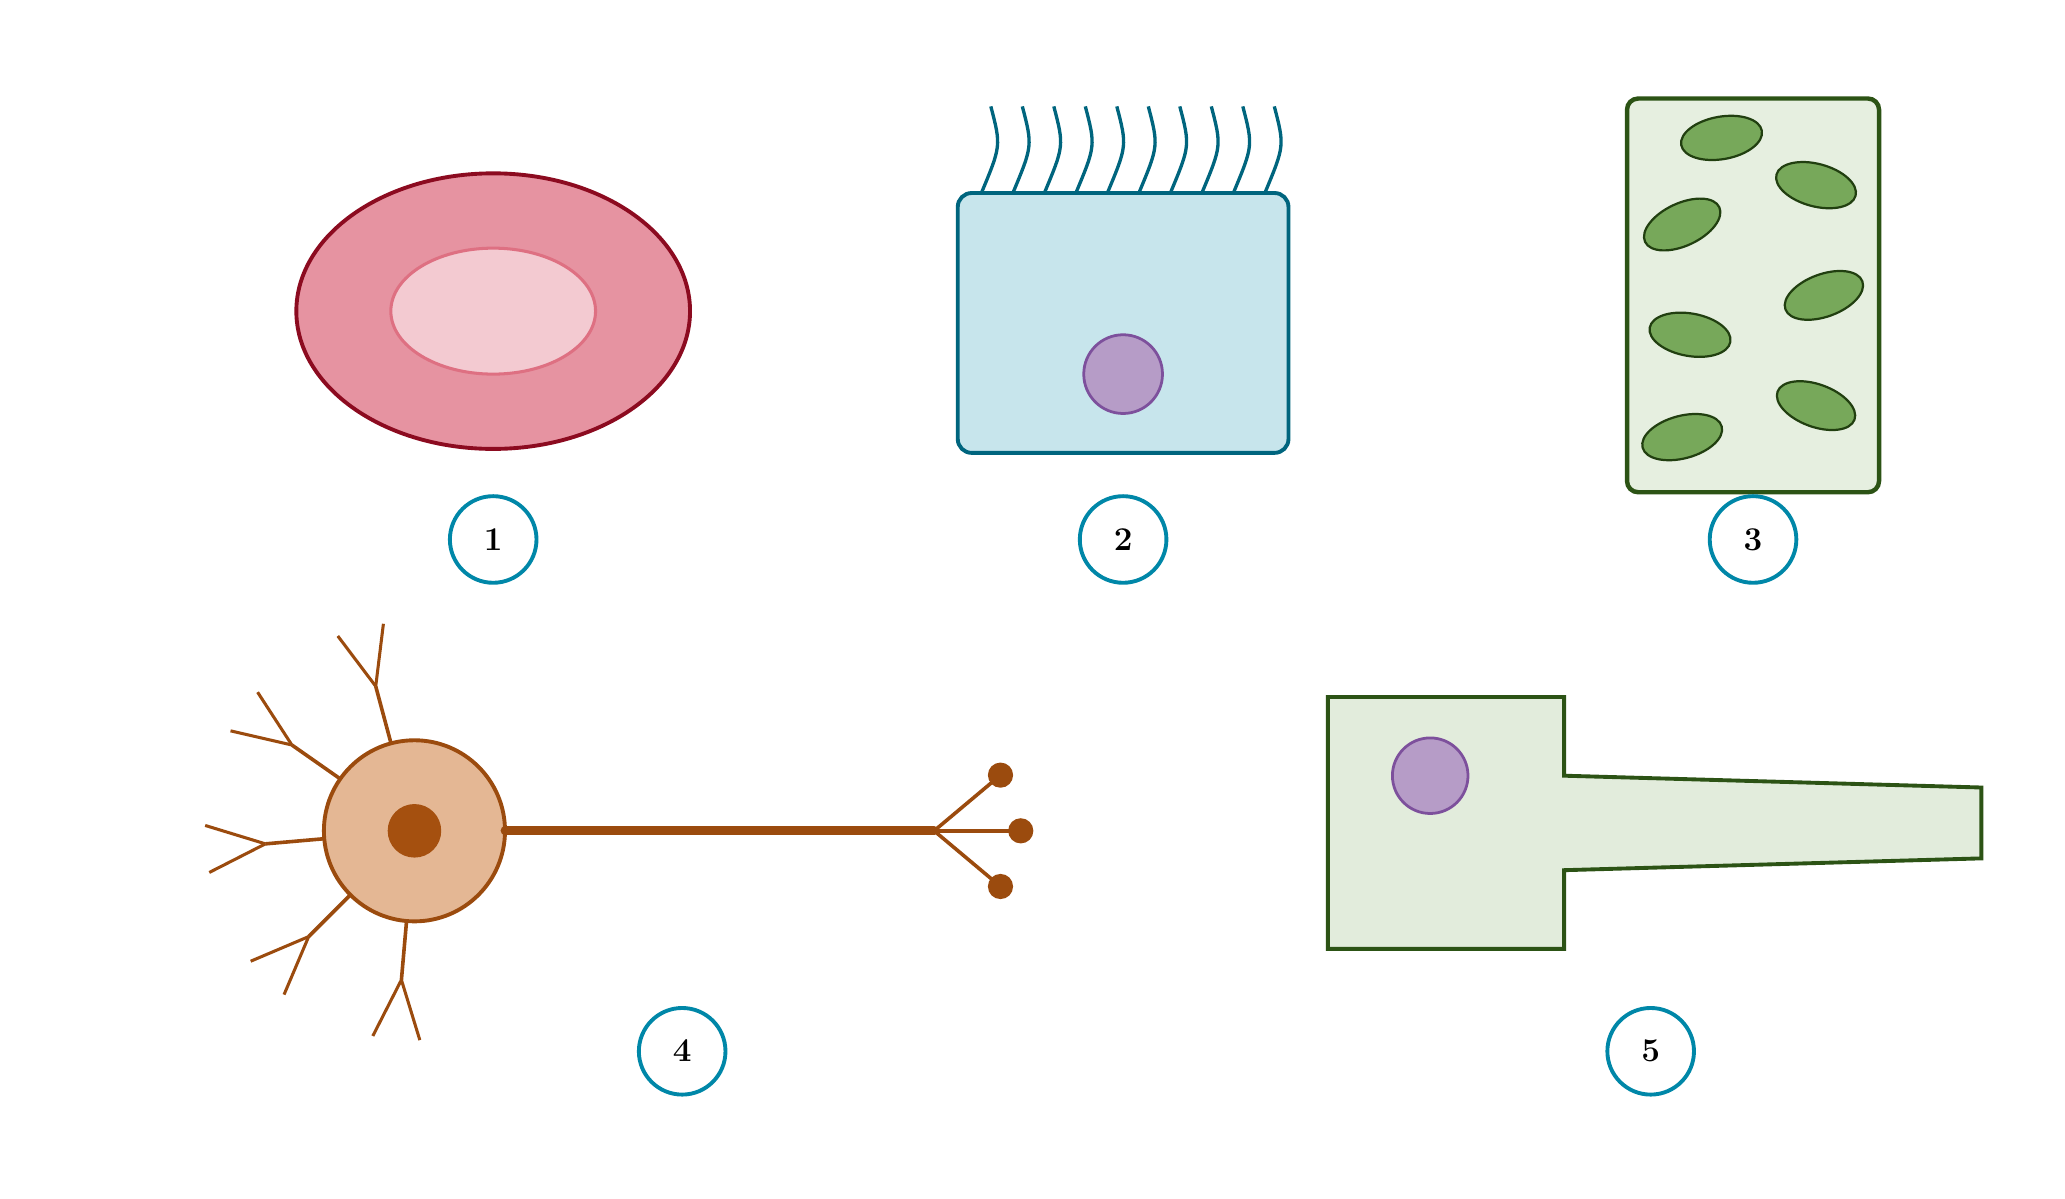
\begin{tikzpicture}[x=1cm,y=1cm,
    num/.style={circle, draw=cbteal, fill=white, line width=1.4pt,
                inner sep=2.4pt, minimum size=11mm, font=\bfseries\large}]

  % ================= row 1: the three compact cells =================

  % ---- 1. red blood cell: a disc seen at an angle, dipped in the middle ----
  \fill[cbred!45] (4,9) ellipse (2.5 and 1.75);
  \draw[line width=1.4pt, cbred!70!black] (4,9) ellipse (2.5 and 1.75);
  \fill[cbred!22] (4,9) ellipse (1.3 and 0.8);
  \draw[line width=1.1pt, cbred!60] (4,9) ellipse (1.3 and 0.8);
  \node[num] at (4,6.1) {1};

  % ---- 2. ciliated cell: a block with moving hairs along the top ----
  \fill[cbteal!22, rounded corners=5pt] (9.9,7.2) rectangle (14.1,10.5);
  \draw[line width=1.4pt, cbteal!75!black, rounded corners=5pt] (9.9,7.2) rectangle (14.1,10.5);
  \foreach \x in {10.2,10.6,...,13.9}{
    \draw[line width=1.2pt, cbteal!75!black]
      (\x,10.5) .. controls (\x+0.25,11.1) .. (\x+0.12,11.6);}
  \fill[cbpurple!45] (12,8.2) circle (0.5);
  \draw[line width=1pt, cbpurple!80] (12,8.2) circle (0.5);
  \node[num] at (12,6.1) {2};

  % ---- 3. palisade cell: a tall box packed with chloroplasts ----
  \fill[cbgreen!14, rounded corners=4pt] (18.4,6.7) rectangle (21.6,11.7);
  \draw[line width=1.6pt, cbgreen!60!black, rounded corners=4pt] (18.4,6.7) rectangle (21.6,11.7);
  \foreach \x/\y/\r in {19.1/7.4/15, 20.8/7.8/-20, 19.2/8.7/-10, 20.9/9.2/20,
                        19.1/10.1/25, 20.8/10.6/-15, 19.6/11.2/10}{
    \begin{scope}[shift={(\x,\y)}, rotate=\r]
      \fill[cbgreen!75] (0,0) ellipse (0.52 and 0.27);
      \draw[line width=0.8pt, cbgreen!45!black] (0,0) ellipse (0.52 and 0.27);
    \end{scope}}
  \node[num] at (20,6.1) {3};

  % ================= row 2: the two long cells =================

  % ---- 4. neurone: body with dendrites, then one long thick axon ----
  \foreach \a in {105,145,185,225,265}{
    \draw[line width=1.3pt, cborange!80!black] (3,2.4) -- ++(\a:1.9);
    \draw[line width=1.1pt, cborange!80!black] (\a:1.9) ++(3,2.4) -- ++(\a+22:0.8);
    \draw[line width=1.1pt, cborange!80!black] (\a:1.9) ++(3,2.4) -- ++(\a-22:0.8);}
  \fill[cborange!45] (3,2.4) circle (1.15);
  \draw[line width=1.4pt, cborange!80!black] (3,2.4) circle (1.15);
  \fill[cborange!85!black] (3,2.4) circle (0.34);
  \draw[line width=3.2pt, cborange!80!black, line cap=round] (4.15,2.4) -- (9.6,2.4);
  \foreach \a in {40,0,-40}{
    \draw[line width=1.3pt, cborange!80!black] (9.6,2.4) -- ++(\a:1.1);
    \fill[cborange!80!black] (\a:1.1) ++(9.6,2.4) circle (0.16);}
  \node[num] at (6.4,-0.4) {4};

  % ---- 5. root hair cell: drawn as ONE outline, so the box and the hair
  %         join with no seam down the middle ----
  \def\roothair{(14.6,0.9) -- (17.6,0.9) -- (17.6,1.9) --
                (22.9,2.05) -- (22.9,2.95) -- (17.6,3.1) --
                (17.6,4.1) -- (14.6,4.1) -- cycle}
  \fill[cbgreen!16] \roothair;
  \draw[line width=1.4pt, cbgreen!60!black] \roothair;
  \fill[cbpurple!45] (15.9,3.1) circle (0.48);
  \draw[line width=1pt, cbpurple!80] (15.9,3.1) circle (0.48);
  \node[num] at (18.7,-0.4) {5};

  \path (-0.4,-1.6) rectangle (23.6,12.6);
\end{tikzpicture}}

\vspace{16pt}
\noindent
\begin{tabularx}{\textwidth}{|c|p{4.4cm}|X|}
  \hline
  \textbf{No.} & \textbf{Name of the cell} & \textbf{Its job} \\
  \hline
  1 \rule[-2.6em]{0pt}{3.5em} & & \\ \hline
  2 \rule[-2.6em]{0pt}{3.5em} & & \\ \hline
  3 \rule[-2.6em]{0pt}{3.5em} & & \\ \hline
  4 \rule[-2.6em]{0pt}{3.5em} & & \\ \hline
  5 \rule[-2.6em]{0pt}{3.5em} & & \\ \hline
\end{tabularx}

% ===========================================================================
% ANSWER KEY (teacher copy only)
% ===========================================================================
\ifkey
\newpage
\hwsection[cbred]{Answer Key --- Teacher Copy}

% The key is for an adult at a desk, not a 12-year-old writing on it.
\linespread{1.0}\selectfont
\setlist[enumerate]{itemsep=2pt, topsep=3pt, leftmargin=*}
\setlist[itemize]{itemsep=2pt, topsep=3pt, leftmargin=*}

\qhead[cbred]{A1}{The four rules}
\noindent (a) $+$, $-$, $-$, $+$. Same signs positive, different signs negative.\\
(b) (a) $-24$ \quad (b) $-21$ \quad (c) $40$ \quad (d) $-6$ \quad (e) $-5$ \quad (f) $8$ \\
\hspace*{1.15em} (g) $0$ \quad (h) $1$ \quad (i) $-56$ \quad (j) $9$ \quad (k) $-25$ \quad (l) $12$

\smallskip
\noindent{\small (g) catches people who reach for a sign rule: zero has no sign, and
anything times zero is zero. (h) is worth a comment too --- a negative divided by
itself is $1$, not $-1$.}

\qhead[cbred]{A2}{Say it, then write it}
\begin{enumerate}[label=\arabic*., itemsep=2pt]
  \item $-7 \times 6 = -42$
  \item $-40 \div 8 = -5$
  \item $-9 \times -4 = 36$
  \item $-35 \div 5 = -7$
  \item $-24 \div 6 = -4$ dollars each
\end{enumerate}
\noindent{\small Question 4 is the reversed-order trap carried over from Homework 1:
``5 divided into $-35$'' is $-35 \div 5$. A student who writes $5 \div -35$ has made
the English error, not an arithmetic one --- make them re-read the sentence rather
than re-do the sum.}

\qhead[cbred]{A3}{A sentence that is only half true}
\noindent (a) $12$ \quad (b) $-7$

\smallskip
\noindent (c) No. It is true for $-3 \times -4$ but false for $-3 + -4$, which is
still negative.

\smallskip
\noindent (d) Anything that attaches the operation, e.g. ``Two negatives make a
positive when you \emph{multiply} or \emph{divide}, but not when you add.''

\smallskip
\noindent{\small This is the whole point of Maths 1.2 and the question most worth
marking properly. Accept any wording that names multiplying and dividing and excludes
adding; reject a (d) that just repeats the original sentence more loudly. If most of
the class gets (c) right and (d) vague, that is a five-minute discussion, not a pile
of red pen.}

\qhead[cbred]{A4}{Brackets, and checking yourself}
\noindent (i) $-3 + -2 = -5$, so $20 \div -5 = -4$ \\
(ii) $-4 + 10 = 6$, so $6 \times -3 = -18$ \\
(iii) $2 - 9 = -7$, so $-6 \times -7 = 42$ \\
(iv) about $-6 \times 4 = -24$ \\
(v) about $64 \div -8 = -8$

\smallskip
\noindent{\small The classic error in (i) is applying the new sign rule inside the
bracket and getting $+5$. The bracket holds an \emph{addition}: two negatives added
stay negative. Watch for it specifically.}

\qhead[cbred]{A5}{Word problems}
\begin{enumerate}[label=\arabic*., itemsep=2pt]
  \item $7 \times -4 = -28$. His balance goes down by 28 dollars.
  \item $-54 \div 6 = -9$, so 9 m downwards each minute.
  \item He loses \textbf{15 dollars}. He sells 0 ducks, so $0 \times 3 = 0$ income and
        $0 \times -2 = 0$ in selling fees --- but the 15-dollar stall fee is charged
        anyway. The 47 and the 3 and the 2 are all decoration.
\end{enumerate}
\noindent{\small Problem 3 is the deadpan one and should be read completely straight.
It is a harder trick than last week's: most of the numbers cancel to zero, but not
\emph{all} of them, so a student who answers ``0'' has stopped one step early. Expect
both ``0'' and ``$-15$'' in the room and make them argue it out.}

\qhead[cbred]{B1}{Build it from the lists}
\noindent (a) 8, 16, 24, 32, 40, 48 \\
(b) 12, 24, 36, 48, 60, 72 \\
(c) 24 and 48 \\
(d) 24

\qhead[cbred]{B2}{Do not just multiply them}
\noindent (a) 21 \quad (b) 20 \quad (c) 24 \quad (d) 9

\smallskip
\noindent (e) 5 divides into 20, so the LCM is just the bigger number, 20. Multiplying
only gives the right answer when the two numbers share no factor --- as in (a), where
$3 \times 7 = 21$ happens to be correct.

\smallskip
\noindent{\small (d) is the deadpan one: both numbers are 9, so there is nothing to
work out. Expect someone to list the multiples of 9 twice before noticing.}

\qhead[cbred]{B3}{Word problems}
\begin{enumerate}[label=\arabic*., itemsep=2pt]
  \item LCM$(6,10) = 30$, so 30 seconds. Not 60 --- 6 and 10 share the factor 2.
  \item LCM$(8,12) = 24$. So 24 sandwiches: \textbf{3 packs of rolls} and
        \textbf{2 packs of cheese}. Students who stop at 24 have done the maths but
        not answered the question; the packs are the point.
\end{enumerate}

\qhead[cbred]{B4}{Now you write the question}
\noindent No single right answer. Check, in this order:
\begin{enumerate}[label=\arabic*., itemsep=2pt]
  \item \textbf{Does it repeat?} (a) needs something happening 7 times, each time
        costing 4 --- a fee, a drop in temperature, a debt. A one-off ``he lost 28
        dollars'' is not a multiplication.
  \item \textbf{Is the sign right?} The $-4$ must be a loss, a fall or a descent, not
        a gain.
  \item \textbf{For (b), are the two things independent and repeating?} Buses, lights,
        alarms, taps, machines. The question must ask when they \emph{next coincide},
        not how many of each.
  \item \textbf{Full sentences, ending in a question?}
  \item \textbf{Does their own answer come out as $-28$, and as 20?}
\end{enumerate}
\noindent{\small One that works for (b): ``One machine in a factory stamps a box every
4 seconds. Another wraps a box every 10 seconds. They have just both finished a box at
the same moment. How many seconds until they finish together again?'' \\
Expect (b) to be much weaker than (a) --- writing a repeating-events story is harder
than writing a repeated-loss one. Worth doing one aloud on the board.}

\qhead[cbred]{C1}{Match the word to its meaning}
\noindent 1--C \quad 2--E \quad 3--A \quad 4--F \quad 5--B \quad 6--D

\qhead[cbred]{C2}{Plant or animal?}
\begin{enumerate}[label=\arabic*., itemsep=2pt]
  \item \textbf{Plant} --- straight, stiff cell walls (and chloroplasts).
  \item \textbf{Animal} --- no cell wall, so no straight edges.
  \item \textbf{Plant} --- every cell has a straight-sided \emph{cell wall}. This is
        the trap. It is Rhoeo leaf epidermis: purple, with no chloroplasts at all,
        because it is not a photosynthesising layer.
  \item \textbf{Animal} --- no cell walls; these are muscle fibres.
\end{enumerate}
\noindent{\small Number 3 catches almost everybody, because they have quietly replaced
``has a cell wall'' with ``is green''. Do not mark it as a careless slip --- it is the
misconception the whole lesson was built to break. Ask them what the onion looked
like: also a plant, also no chloroplasts.}

\qhead[cbred]{C3}{Similar is not the same}
\begin{enumerate}[label=\arabic*., itemsep=2pt]
  \item \ldots both of them have a cell membrane, cytoplasm, a nucleus and
        mitochondria. (Any of those four.)
  \item \ldots a plant cell has a cell wall (or chloroplasts, or a sap vacuole), but
        an animal cell does not.
  \item An animal cell has no cell wall, so there is nothing stiff to hold it in a
        fixed shape --- only the thin, flexible cell membrane.
\end{enumerate}
\noindent{\small The word to police here is \emph{similar}. A student who writes ``they
are the same'' has lost the distinction the lesson taught, even if the rest of the
sentence is right.}

\qhead[cbred]{C4}{Put the method in order}
\noindent Reading down the table as printed: \textbf{3, 5, 1, 6, 4, 2}.

\smallskip
\noindent In order: (1) rub the inside of your cheek with a cotton bud; (2) wipe it
onto the middle of a clean slide; (3) add a drop of methylene blue stain; (4) lower a
cover slip slowly to avoid bubbles; (5) looking from the side, move the lens down
close to the slide; (6) look down the eyepiece and focus by moving the lens away.

\smallskip
\noindent Why from the side: with your eye at the eyepiece you cannot judge the gap,
so looking from the side is the only way to avoid driving the lens through the slide.

\smallskip
\noindent{\small Focusing \emph{away} from the slide, never towards it, is the same
safety point said twice. Accept either the safety answer or ``so you do not break the
slide or the lens''.}

\qhead[cbred]{D1}{Finish the table}
\noindent
\begin{tabularx}{\linewidth}{@{}p{2.4cm}p{3.4cm}p{3.6cm}X@{}}
  \textbf{Neurone} & carries electrical signals & a very long axon; short dendrites &
  signals travel far and fast; dendrites collect them \\
  \textbf{Ciliated} & sweeps mucus away from the lungs & tiny moving hairs (cilia) &
  they sweep the mucus, with its trapped dust and germs, along \\
  \textbf{Root hair} & absorbs water from the soil & a long, thin extension &
  a big surface area, so water moves in easily \\
  \textbf{Palisade} & makes food by photosynthesis & packed with chloroplasts, near
  the top of the leaf & catches as much sunlight as possible \\
\end{tabularx}

\qhead[cbred]{D2}{Use the sentence, and think}
\begin{enumerate}[label=\arabic*., itemsep=2pt]
  \item ``A root hair cell is adapted to absorb water because it has a long, thin
        extension that gives it a big surface area.''
  \item ``A palisade cell is adapted to make food by photosynthesis because it has
        many chloroplasts.''
  \item \textbf{Cytoplasm} and a \textbf{cell membrane}. \emph{Not} a nucleus --- the
        red blood cell has none. Accept ``they are all specialised'' as a third.
  \item Roots are underground in the dark, and chloroplasts need sunlight to make
        food, so they would be useless there.
\end{enumerate}
\noindent{\small Question 3 is the precision point of Science 1.3, and nearly everyone
writes ``a nucleus''. Let them, then ask what a red blood cell gave up to fit more
haemoglobin in. In 1 and 2, mark the \emph{frame} as much as the content: if
``adapted to'' and ``because it has'' are both missing, the science may be right but
the sentence is not the one being taught.}

\qhead[cbred]{D3}{Name the cell}
\noindent 1 --- red blood cell (carries oxygen) \\
2 --- ciliated cell (sweeps mucus away from the lungs) \\
3 --- palisade cell (makes food by photosynthesis) \\
4 --- neurone (carries electrical signals) \\
5 --- root hair cell (absorbs water from the soil)

\smallskip
\noindent{\small 2 and 5 are the pair most often swapped: both are drawn as a box with
something sticking out of it. The cilia are \emph{many} short hairs on the top; the
root hair is \emph{one} long extension from the side. \\
If anyone labels the pale middle of 1 as a nucleus, that is the misconception from
D2.3 showing up again --- a red blood cell has no nucleus, and the pale patch is the
dip in the disc.}

\fi

\end{document}
